\chapter{Physical and numerical model}
\label{s:model}
%
\section{General}
%
In this chapter the problems that \NAME solves approximately are discussed, describing
the governing equations, and the numerical model used so in order that users
and developers can refer to this chapter in order to know what \NAME is solving.\rc
%
The algorithmic details are exposed later, in chapter \ref{s:aquagpusph}.\rc
%
\NAME is a highly modable software\footnote{The functionality, or even the equations solved,
can be modified through OpenCL scripts modification}, so the numerical model presented here
corresponds to the standard provided software.
%
\section{Governing equations}
\label{ss:governing_equations}
%
\subsection{Field equations}
%
\NAME uses weakly-compressible SPH (formerly WCSPH or W-SPH) method in
order to approximate the solution of the incompressible Navier-Stokes
equations, but since it is a highly modable software, you can adapt it to
approximate different equations. In this formulation the incompressibility
is sought by modelling the flow with a compressible fluid which, in
the flow regime expected, presents very small density fluctuations.
The fluid is assumed to be barotropic which implies that the internal energy
equation is decoupled from the continuity and momentum equations.\rc
%
The compressible Navier-Stokes equations for a barotropic fluid in Lagrangian
formalism are:
%
\begin{eqnarray}
	\label{eq:governing_eqns:field_eqns:continuity}
	\dsty{\frac{D \rho}{D t}} & = & -\rho \, \divergence(\bs{u}) \vspace{0.3cm} \\
	\label{eq:governing_eqns:field_eqns:momentum}
	\dsty{\frac{D \bs{u}}{D t}} & = & \bs{g} \, + \, \dsty{\frac{\divergence(\varmathbb{T})}{\rho}}
	\vspace{0.3cm} \\
	\label{eq:governing_eqns:field_eqns:eos}
	p & = & p(\rho)
\end{eqnarray}
%
Where (\ref{eq:governing_eqns:field_eqns:continuity}) is referenced to as
continuity or mass conservation equation,
(\ref{eq:governing_eqns:field_eqns:momentum}) as the linear momentum
conservation one, and (\ref{eq:governing_eqns:field_eqns:eos}) as the equation
of state (EOS).\rc
%
\citet{monaghan_arfm_2012} discuss the properly EOS for weakly compressible
simulations, purposing an equation such that:
%
\begin{eqnarray}
\label{eq:governing_eqns:field_eqns:eos:arfm_2012}
p  =  p_0 \, + \, \dsty{\frac{c_s^2 \rho_0}{\gamma}} \left( \left( \dsty{\frac{\rho}{\rho_0}} \right)^{\gamma} - 1 \right)
\end{eqnarray}
%
In the introduced equations $\rho$ is the fluid density, $\rho_0$ is the
reference density, $p$ is the pressure, $p_0$ is the ambient pressure, $c_s$ is
the sound velocity and $\bs{g}$ is a generic external volumetric force field. A
specific equation of state (EOS) has been selected. Sound speed $c_s$ will be
chosen high enough to get density variations below a certain limit.\rc

The flow velocity, $\bs{u}$, is defined as the material derivative of a fluid
particle position $\bs{r}$:
%
\begin{eqnarray}
\frac{D \bs{r}}{D t} \, = \, \bs{u}
\end{eqnarray}
%
$\varmathbb{T}$ is the stress tensor of a Newtonian fluid:
%
\begin{eqnarray}
\varmathbb{T}  \, = \, \left(\, - p \, + \, \lambda \, \textrm{tr}\,  \varmathbb{D} \,\right) \, \mathds{1}  \,+  \,2 \, \mu \, \varmathbb{D} \,,
\end{eqnarray}
%
with $\varmathbb{D}$ being the rate of strain tensor, i.e. $\varmathbb{D} = ( \nabla \bs{u} + \nabla \bs{u}^{T} )/2$.\rc
%
Finally, $\mu$ and $\lambda$  are the viscosity coefficients. \rc
%
Other formulations can be found in order to compute fully incompressible SPH, but
WCSPH has the great advantage that an explicit time integrator can be used to
advance in time, and hence no linear system of equations has to be solved in order to get
the pressure field at each time step.
%
\subsection{Boundary conditions}
%
Denoting the fluid domain by $\Omega$, and the boundary by $\partial \Omega$,
boundary conditions can be separated in those to be applied on solid boundaries,
$\partial \Omega_B$, and on free surfaces, $\partial \Omega_F$, as shown in the
figure \ref{fig:aquagpusph:BC}.
%
\subsubsection{Solid boundary conditions}
%
In the solid boundaries, an unpenetrability condition must be imposed, meaning that
%
\begin{eqnarray}
\bs{u}_n(\bs{x}) = \bs{V}_n(\bs{x}) \qquad \forall \bs{x} \in \partial\Omega_B
\end{eqnarray}
%
where $\bs{u}_n$ is the fluid velocity projected over the solid normal at point
$\bs{x}$, and $\bs{v}_n$ is the solid velocity projected over the solid normal.\rc
%
Regarding to the tangential velocity on the solid, a no-slip condition can be imposed:
%
\begin{eqnarray}
\bs{u}_t(\bs{x}) \big\vert_{\mathrm{no-slip}} = \bs{V}_t(\bs{x})  \qquad \forall \bs{x} \in \partial\Omega_B
\end{eqnarray}
%
where $\bs{u}_t$ and $\bs{v}_n$ are the fluid velocity and solid velocity
respectively, both of them projected on the solid tangent. But in some cases Free slip
boundary condition can be used, letting that tangential velocity at solid be freely
computed.
%
\subsubsection{Free surface boundary conditions}
%
Along the free surface a kinematic and a dynamic boundary conditions must be satisfied.
The kinematic boundary condition implies that material points already on the free surface
must remain in $\partial \Omega_F$ as this region evolves with the fluid flow.
%
\begin{eqnarray}
\bs{u}_n(\bs{x}) = \bs{V}_n(\bs{x}) \qquad \forall \bs{x} \in \partial\Omega_F
\end{eqnarray}
%
The dynamic free-surface BC is a consequence of the continuity of the stresses across
the free surface. Assuming that surface tension is negligible, a free surface does not
stand neither perpendicular normal stresses nor parallel/tangential shear stresses.
For a Newtonian fluid, by denoting such stress field as $\bs{t}$, 
the dynamic free-surface BC can be expressed as:
%
\begin{eqnarray}
\bs{t} \, = \, \varmathbb{T} \cdot \bs{n} \, = \, \left(\, - p \, + \, 
\lambda \, \textrm{tr}\,  \varmathbb{D} \,\right) \, \bs{n}    \, + \,
2 \, \mu \, \varmathbb{D} \cdot \bs{n} \, = \, 0 \,.
\end{eqnarray}
%
\begin{figure}[!ht]
  \centering
  \includegraphics[width=0.4\textwidth]{BC}
  \caption{Boundary conditions scheme}
  \label{fig:aquagpusph:BC}
\end{figure}
%
\subsection{Initial conditions}
%
Since the governing equations \ref{eq:navierstokes} corresponds to an hyperbolic problem,
that must be solved as an initial value problem, the pressure, density and velocity fields
(right hand sides of the equations involved fields) must be known at a initial time $t_0$
where a forward time integration will be performed. In this type of problems backward
time integration is not generally possible.\rc
%
The fields in the initial condition must accomplish the governing equations
\ref{eq:navierstokes}. If the fluid is in rest continuity equation is implicitly
accomplished due to the velocity is null, but fields must be selected in order to get null
accelerations from momentum equation.
%
\section{SPH approximation}
\label{ss:sph_description}
%
\subsection{General}
%
SPH (Smoothed Particle Hydrodynamics) is a numerical method of simulation created at 1977
independently by Lucy (1977) and Gingold \& Monaghan (1977). In this method the fluid is
divided into a set of particles for which the fluid equations are written in a Lagrangian
form, avoiding mesh requirement. Meshfree character of the method is the most attractive
feature because it can be applied to really complex geometries where a mesh generation is not
a good option.\rc
%
SPH was presented as an application of the Monte Carlo method for the resolution of problems
of gas dynamics on astrophysics, but was extended to incompressible flows by Monaghan (1994).
%
\subsection{Continuous model}
\label{ss:sph_continuous}
%
In SPH a kernel $W_h(\bs x)$ is defined as an even function such that
%
\begin{eqnarray}
\int_{-\infty}^{\infty} W_h(\bs y) d\bs y = 1
\end{eqnarray}
%
For practical purposes, the defined kernel $W_h(\bs x)$ vanishes for $\left\vert \bs x \right\vert > sh$,
where $s$ is an integer greater than 0. In \NAME
the \citet{wendland_1995} purposed kernel is mainly used, but other ones are supported and can be selected
with minor changes in the OpenCL code. In table \ref{tables:abstract:kernels} a list with the provided
kernels can be found, but the user can incorporate easily other kernels.\rc
%
The SPH approximation with respect to the kernel $W_h(\bs x)$ of a scalar or vector function $f(\bs x)$
is defined as
%
\begin{eqnarray}
\langle f \rangle (\bs{x}) := \frac{1}{\gamma_h(\bs{x})} \SPHint f(\bs{y}) W_h(\bs{x}-\bs{y}) d\bs{y}
\end{eqnarray}
%
where $\gamma_h(\bs x)$ is the Shepard normalization factor, defined as
%
\begin{eqnarray}
\gamma_h(\bs x) := \SPHint W_h(\bs x - \bs y) d\bs y
\end{eqnarray}
%
with $\Omega$ as the ball of radius $sh$ centred on $\bs x$, subtracting eventually the domain out
of fluid. In the standard SPH formulation Shepard normalization factor is neglected, considering
it $\gamma_h(\bs x) = 1$, that is a good approach far enough of the solid boundary, or near too
if fluid extension based boundary conditions are imposed. Shepard correction can produce some
instabilities, but improves the consistency and is mandatory for De Leffe's type boundary condition
\citep{deleffe_etal_spheric09,ferrand_etal_2012}, that will be discussed later. On the other hand
droping if from the formulation makes it intrinsically conservative \citep{mon2005}, that could be
a really desirable property.\rc
%
The gradient and the divergence of functions can be also interpolated
%
\begin{eqnarray}
\langle \gradient p \rangle (\bs x) = \frac{1}{\gamma_h(\bs x)} \SPHint \gradient p(\bs y) W_h(\bs x - \bs y) d\bs y
\end{eqnarray}
\begin{eqnarray}
\langle \divergence(\bs{u}) \rangle (\bs x) = \frac{1}{\gamma_h(\bs x)} \SPHint \divergence(\bs{u}(\bs y)) W_h(\bs x - \bs y) d\bs y
\end{eqnarray}
%
In these formulas $\gradient p$ and $\divergence(\bs{u})$ are not known. Integrating by parts the
differential operators can be conveniently moved to the kernel function. We will work only over the gradient
operator to show the procedure but analogous treatment is applied to the divergence one.
%
\begin{eqnarray}
\langle \gradient p \rangle (\bs x) = \frac{1}{\gamma_h(\bs x)} \left(
	  \SPHint \gradient \left( p(\bs y) W_h(\bs x - \bs y) \right) d\bs y
	- \SPHint p(\bs y) \gradient W_h(\bs x - \bs y) d\bs y
\right)
\end{eqnarray}
%
If $W_h(\bs x)$ is an even function, $\gradient W_h(\bs x)$ is an antisymmetric one, so we can use
this property to switch the integral terms signs. Also we can use the divergence theorem over the first
integral term.
%
\begin{eqnarray}
\langle \gradient p \rangle (\bs x) = \frac{1}{\gamma_h(\bs x)} \left(
	  \SPHint p(\bs y) \gradient W_h(\bs y - \bs x) d\bs y
	- \SPHboundint p(\bs y) W_h(\bs y - \bs x) \bs n(\bs y) dS(\bs y)
\right)
\end{eqnarray}
%
Where $\partial \Omega$ denotes the boundary of $\Omega$. The contour term has been traditionally neglected
in the literature because authors assume that $p = 0 \in \partial \Omega$\footnote{The almost used boundary
conditions along the solid walls in SPH have consists in fluid extensions, so the contour $\partial \Omega$
has been rely only for the free surface}. In \NAME this boundary integral and the Shepard correction term
can be retained.\rc
%
Regarding Laplacian operator, The 2 most popular formulations to approximate it are
\citet{Monaghan+Gingold:83} form and \citet{Morris+etal:1997} form. \citet{Colagrossi2009} demonstrated that
only the first one provides right dissipation in the presence of a free surface when boundary terms are
discretized, so in \NAME the second way has not been implemented.\rc
%
Assuming that the viscosity coefficients are constant all over the fluid domain, the continuous
formulation of the Monaghan viscous term is:
%
\begin{eqnarray}
\langle \laplacian \bs u \rangle (\bs x) = 
\frac{\mu \, K}{\gamma_a(\bs x) \, \rho(\bs x)} \SPHint
	\frac{
		\left(\bs{u}(\bs y) - \bs{u}(\bs x) \right) \cdot (\bs{y} - \bs{x})
	}{
		\left\vert \bs{y} - \bs{x} \right\vert^2
	} \, \gradient  W_h(\bs y - \bs x) \, d\bs{y}
\end{eqnarray}
%
where $K$ is a parameter depending on the spatial dimension ($K\,=\,6,8,15$, respectively in $1D$,
$2D$ and $3D$).\rc
%
This viscous term is valid far enough of the boundary, and provides right dissipation near the free surface.
Boundary viscous term is added as described by \citet{Maciaetal_PTP_2012} in order to can impose no-slip
boundary conditions in the boundaries.
%
\begin{eqnarray}
\begin{array}{lcl}
\langle \laplacian \bs u \rangle (\bs x) & = &
\dsty{\frac{\mu}{\gamma_a(\bs x) \, \rho(\bs x)}} \left(
	\SPHint K \frac{
		\left(\bs{u}(\bs y) - \bs{u}(\bs x) \right) \cdot (\bs{y} - \bs{x})
	}{
		\left\vert \bs{y} - \bs{x} \right\vert^2
	} \, \gradient  W_h(\bs y - \bs x) \, d\bs{y} \right.
	\vspace{0.3cm} \\ & & 	
    \left. - \dsty{\SPHboundint \left(\bs{u}(\bs y) - \bs{u}(\bs x) \right) \frac{
		 (\bs{y} - \bs{x}) \cdot \bs{n}(\bs{y})
	}{
		\left\vert \bs{y} - \bs{x} \right\vert^2
	} \, W_h(\bs y - \bs x) \, dS(\bs{y})}
    \right)
\end{array}
\end{eqnarray}
%
All this smoothing procedures introduces errors in the representation of functions and operators. These errors
goes to zero as $h \rightarrow 0$, but the convergence order may be different
\citep{MaciaetalPTP,Maciaetal_PTP_2012}.
%
\begin{table}[h!b!p!]\small
	\centering
	\begin{tabular}{| c | c | c | l | }
		\hline
		\cellcolor[rgb]{0.7,0.7,0.7}Kernel & \cellcolor[rgb]{0.7,0.7,0.7}Support \\
		\hline
		Wendland     & $2h$ \\
		\hline
		Cubic spline & $2h$ \\
		\hline
		Gaussian     & $3h$ \\
		\hline
	\end{tabular}
	\caption{\NAME provided kernels.}
	\label{tables:abstract:kernels}
\end{table}
%
\subsection{Discretized model}
\label{ss:sph_discretized}
%
For practical purposes the integrals present on continuous SPH interpolation are solved numerically,
so another error must be considered due to the discretization \citep{Quinlan_06,Amicarelli2011279}.
In order to do it, the space will be discretized placing a set of particles that is treated in a
Lagrangian point of view. $d\bs{y}$ must be then discretized as the volume of the particles, that can
be rewritten such that
%
\begin{eqnarray}
d\bs{y} \approx \frac{m_b}{\rho_b}
\end{eqnarray}
%
allowing us to discretize the operators.
%
\begin{eqnarray}
\label{eq:sph:gradient}
\langle \gradient p \rangle_a = \frac{1}{\gamma_a} \left(
	  \sum\limits_{b \in \mathrm{Fluid}} \frac{p_b}{\rho_b} \gradient W_{ab} m_b
	- \sum\limits_{b \in \mathrm{Boundary}} p_b W_{ab} \bs{n}_b S_b
\right)
\end{eqnarray}
%
In the equation \ref{eq:sph:gradient} the discretized version of the SPH gradient operator over the pressure
field is shown, where the value is computed interpolating it from the neighbour particles and, eventually,
from the neighbour wall elements.\rc
%
In the figure \ref{fig:sph:interpolationscheme} a scheme about the interpolation over a particle labelled
``$a$'' is shown, the index $b$ of the first sum moves along all the fluid particles, but since the kernel
nullifies at a distance $s \, h$, only the particles near enough will be considered.\rc
%
In the figure \ref{fig:sph:wendland} 2D Wendland kernel value is shown. Both kernel value $W$ and
gradient value $\gradient W$ nullifies for distances $\vert \bs{x} \vert > 2 \, h$. Must be noticed that
$\gradient W$ nullifies also for $\vert \bs{x} \vert = 0 \, \mbox{m}$, but not the kernel value.\rc
%
As introduced previously, the weight function $W$ is even, but the gradient $\gradient W$ is an odd
function.\rc
%
In the same way Laplacian operator can be also discretized:
%
\begin{eqnarray}
\begin{array}{lcl}
\langle \laplacian \bs u \rangle_a & = & 
\dsty{\frac{\mu}{\rho_a \, \gamma_a}} \left(\dsty{
    \sum\limits_{b \in \mathrm{Fluid}}
	K \frac{
		\left(\bs{u}_b - \bs{u}_a \right) \cdot (\bs{x}_b - \bs{x}_a)
	}{
		 \rho_b \, \left\vert \bs{x}_b - \bs{x}_a \right\vert^2
	} \, \gradient  W_{ab} \, m_b }\right.
    \vspace{0.3cm} \\ & & \left.\dsty{
    \sum\limits_{b \in \mathrm{Boundary}}
	\left(\bs{u}_b - \bs{u}_a \right)
	\frac{
		 (\bs{x}_b - \bs{x}_a) \cdot \bs{n}_b
	}{
		 \left\vert \bs{x}_b - \bs{x}_a \right\vert^2
	} \, W_{ab} \, S_b}\right)
\end{array}
\end{eqnarray}
%
Since the divergence operator is so quite similar to the gradient, is not introduced here due to will
be discussed a little bit more in the following section.\rc
%
So in the SPH discretized model 2 main spatial variables must be selected:
%
\begin{enumerate}
	\item Kernel height $h$: Set the ball where values will be taken in order to perform the smoothed
	interpolation. as this value goes to zero, the weight function converges to the Dirac's delta one,
	so converges to the real solution as well.
	\item Distance between particles $r$: Set the resolution of the numerical integrals approximation,
	so in the limit of $r \rightarrow 0 \, \mbox{m}$, the integrals are exactly computed.
\end{enumerate}
%
Since $r$ must be lower than interaction distance $s \, h$, usually this 2 key values are changed by $h$
and $h / r$ (formerly $h_{fact}$), or by $r$ and $h / r$\footnote{In \NAME this second approach is applied}.
The kernel height defines the problem resolution therefore, and decreasing this value the number of particles
increase improving the result resolution as values smoothed interpolation (considering that $h_{fact}$ is
preserved constant). The distance between particles, expressed as the ratio $h / r$, defines the number
of neighbours that will interact with each particle, so increasing this value the number of interactions
will increase, and the integrals approximation will be improved.
%
\begin{eqnarray}
\lim_{h \to 0; \, \frac{h}{r} \to \infty} \langle p \rangle = p
\end{eqnarray}
%
The problem complexity is $\mathrm{f} \left((1/h)^3 \,\cdot\, (h/r)^3\right)$ for a $3D$ simulation (time
integration associated complexity is not considered yet) therefore.
%
\begin{figure}[!ht]
  \centering
  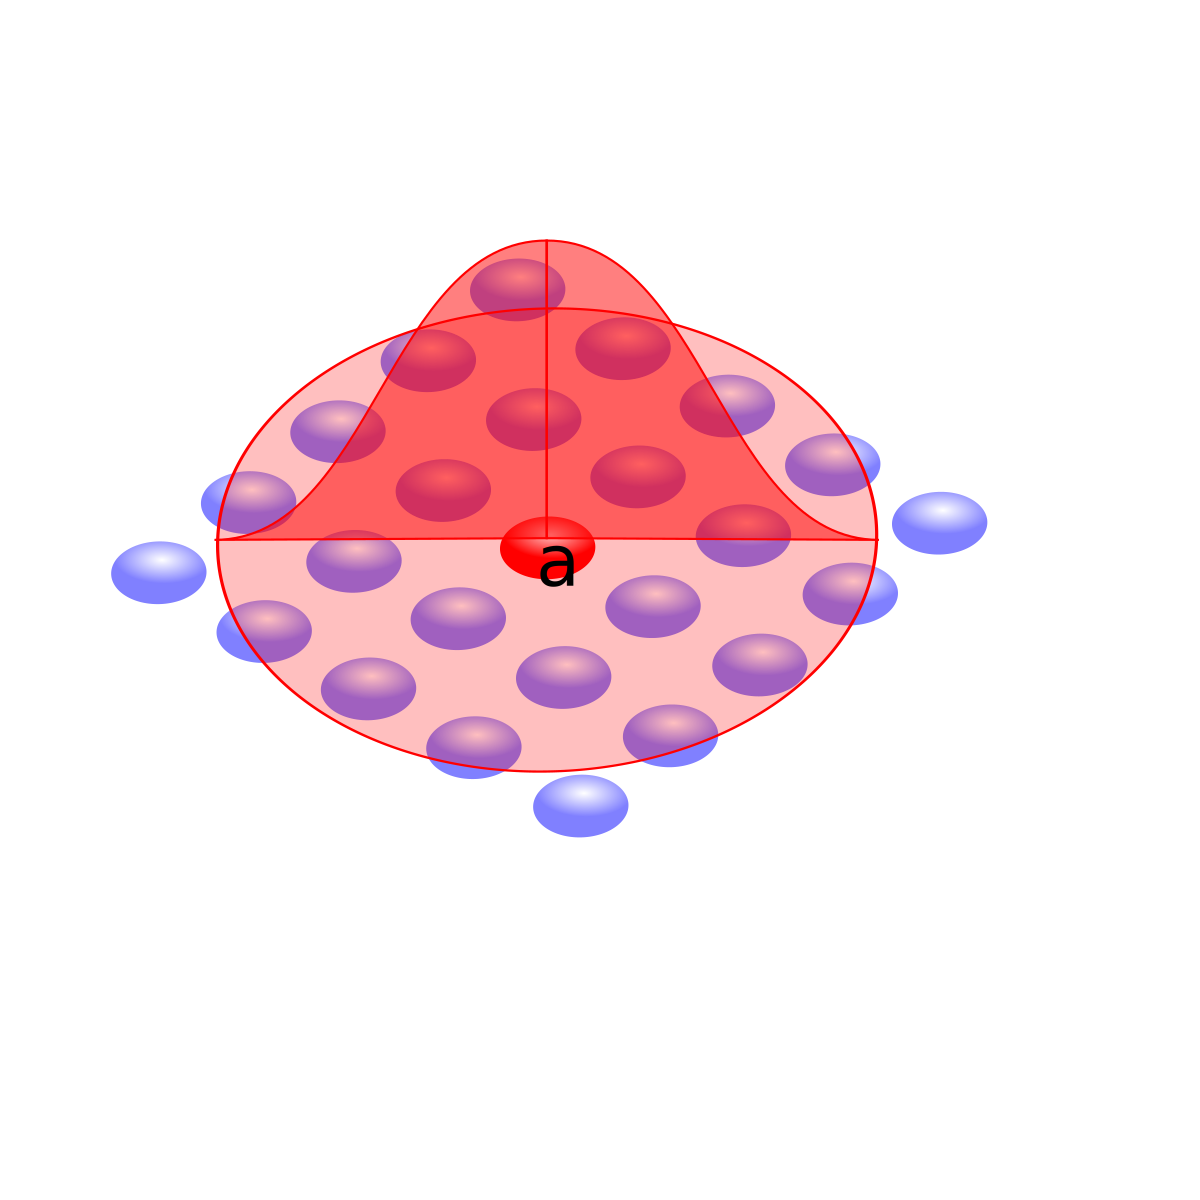
\includegraphics[width=0.5\textwidth]{SPHInterpolation}
  \caption{Discrete SPH interpolation scheme}
  \label{fig:sph:interpolationscheme}
\end{figure}
%
\begin{figure}[!ht]
  \centering
  \includegraphics[width=0.8\textwidth]{wendland/wendland2D}
  \caption{2D Wendland Kernel value (and gradient), $h=1 \mbox{m}$}
  \label{fig:sph:wendland}
\end{figure}
%
\subsection{\NAME discretized operators used}
\label{ss:intro:aquagpusph:operators}
%
For conservation considerations, that you can find on \citep{mon2005} and
\citep{Colagrossi2009}, the operators used in \NAME are not the shown on previous
section, but are conveniently modified (formerly simmetrized) as
%
\begin{eqnarray}
\label{eq:aquagpusph:operators}
\begin{array}{lcl}
\dsty{\left\langle \frac{\gradient p}{\rho} \right\rangle_a} & = & 
\dsty{\frac{1}{\gamma_a}} \left(\dsty{
	\sum\limits_{b \in \mathrm{Fluid}}
		\left(\frac{p_a}{\rho_a^2} + \frac{p_b}{\rho_b^2}\right)
	\gradient W_{ab} m_b}\right.
	\vspace{0.1cm} \\ & & \left.\dsty{
	- \sum\limits_{b \in \mathrm{Boundary}}
		\rho_b \left(\frac{p_a}{\rho_a^2} + \frac{p_b}{\rho_b^2}\right)
	 W_{ab} \, \bs{n}_b \, S_b}\right)
\vspace{0.3cm} \\

\dsty{\left\langle \rho \, \divergence(\bs{u}) \right\rangle_a} & = & 
\dsty{\frac{1}{\gamma_a}} \left(\dsty{
	\sum\limits_{b \in \mathrm{Fluid}}
		\left(\bs{u}_b - \bs{u}_a\right)
	\gradient W_{ab} m_b}\right.
	\vspace{0.1cm} \\ & & \left.\dsty{
	- \sum\limits_{b \in \mathrm{Boundary}}
		\rho_b \left(\bs{u}_b - \bs{u}_a\right) \cdot n_b
	 W_{ab} \, S_b}\right)
\vspace{0.3cm} \\

\langle \laplacian \bs u \rangle_a & = & 
\dsty{\frac{\mu}{\rho_a \, \gamma_a}} \left(\dsty{
    \sum\limits_{b \in \mathrm{Fluid}}
	K \frac{
		\left(\bs{u}_b - \bs{u}_a \right) \cdot (\bs{x}_b - \bs{x}_a)
	}{
		 \rho_b \, \left\vert \bs{x}_b - \bs{x}_a \right\vert^2
	} \, \gradient  W_{ab} \, m_b }\right.
    \vspace{0.1cm} \\ & & \left.\dsty{
    \sum\limits_{b \in \mathrm{Boundary}}
	\left(\bs{u}_b - \bs{u}_a \right)
	\frac{
		 (\bs{x}_b - \bs{x}_a) \cdot \bs{n}_b
	}{
		 \left\vert \bs{x}_b - \bs{x}_a \right\vert^2
	} \, W_{ab} \, S_b}\right)
\end{array}
\end{eqnarray}
%
The operators shown above results from the divergence theorem application over the
operators to interpolate, and have the main advantage that are ever convergent for
constant fields (of pressure and velocity).\rc
%
Weakly compressible SPH formulation carry some high frequency pressure oscillations
caused by the small density fluctuations with the huge incompressibility requirements.
In order to solve partially this effect the density field, that results from a
evolution process, can be reinitialized from particles positions using the property
%
\begin{eqnarray}
\dsty{\left\langle \rho \right\rangle_a} =  
\dsty{\frac{1}{\gamma_a}} \dsty{ \sum\limits_{b \in \mathrm{Fluid}} W_{ab} m_b}
\end{eqnarray}
%
That allows to recover a smooth density field. This correction is not usually
recommended due to can carry some instabilities, but when applied, in almost cases
this correction is only used letting some time steps between corrections. In \NAME
you can select how many steps must run before apply this correction, or simply don't
apply it.
%
\subsection{Boundary conditions}
%
\subsubsection{Free surface boundary conditions}
%
Free surface kinematic and dynamic boundary conditions are automatically accomplished
in the W-SPH formulation, so only the consistency of the operators must be guaranteed.
%
Considering null the ambient pressure $p_0$ in the state equation of the governing
ones \ref{eq:navierstokes} no pressure extra condition has to be imposed at the free
surface as \citet{Colagrossi2009} demonstrates.\rc
%
Unfortunately near the free surface gradient, divergence an Laplacian operators shown in the
equations \ref{eq:aquagpusph:operators} are convergent, but not consistent due to the
result converges to a wrong value. The half good news is that, since the results converges,
and the region where the results are inconsistent is confined to a distance $s \, h$ of
the free surface, in a integral point of view the operators introduced converges to the
right solution with order $\mathcal{O}(h)$.\rc
%
In order to get consistent gradient, divergence an Laplacian operators near the free surface,
as the most desirable ones, track process over the free surface is needed, with a significant
regression in the computational efficiency and robustness.\rc
%
So, assuming an inconsistency near the free surface that is bounded, with an ambient pressure
such that $p_0 = 0 \, \mbox{Pa}$, no additional conditions needs to be imposed in the free
surface therefore.\rc
%
All these assumptions are refereed to monophasic simulations, that are the mainly used in \NAME
simulations.
%
\subsubsection{Solid boundary conditions}
\label{ss:sph:discrete:BC}
%
Regarding solid body boundary conditions \NAME allows to use most popular SPH to modeling techniques:
%
\begin{enumerate}
	\item \textbf{Fixed particles}: Also known as dummy particles, this method consists
	of extending the fluid domain across the wall with fluid particles, fixing their motion.
	This is the boundary condition traditionally used on SPH method.
	\item \textbf{Ghost particles}: This method consist on extending the fluid domain across
	the wall as well, but in this case the fluid at the other side is obtained as mirroring
	process over the fluid domain. It has been developed as an improvement of the previous one.
	\item \textbf{Elastic bounce}: In this method the particles near to the wall, that will
	trespass it, are treated with an elastic bounce model, where an elastic bounce factor is
	used to set the amount of energy conserved in the interaction. This boundary condition
	is not designed to use it alone, but can be mixed with the other ones in order to can
	manage the particles that will cross over the walls without crashing the simulation.
	\item \textbf{Boundary integrals}: Introduced by \citet{deleffe_etal_spheric09},
	and formalized by \citet{ferrand_etal_2012}, in this method the boundary integrals
	are numerically solved along the walls. Is the most recent one, but the consistency
	has been probed by \citet{Maciaetal_PTP_2012}, with the examples performed with \NAME
	software.
\end{enumerate}
%
Each boundary condition type has some advantages, and some combinations of them can be applied in
your simulations. Boundary conditions introduced are described and discussed in detail at section
\ref{ss:aquagpusph:boundaries}, where their algorithmic details are discussed.
%
\subsection{Initial condition}
\label{ss:sph:discrete:initialconditions}
%
As introduced in section \ref{ss:sph_discretized}, you must provided a set of particles in the
initial time instant $t_0$. The initial condition must accomplish the governing equations
\ref{eq:navierstokes}. The most frequently used initial condition is a fluid in rest, so we are
focused in this particular case, describing the process to generate the particles.\rc
%
Since the fluid is in rest, and velocity is null therefore, so the continuity equation is implicitly
accomplished. Regarding the momentum equation, if a volumetric force exist (for instance the gravity
force), a pressure gradient must be forced in order to get null accelerations (formerly known as the
hydrostatic pressure), such that
%
\begin{eqnarray}
p = p_0 + \rho_0 \, \bs{g} \cdot \bs{z}
\end{eqnarray}
%
Where $p_0 = 0 \, \mbox{Pa}$, and $z = 0 \, \mbox{m}$ in the free surface. But the state equation impose
a relation between the density field and the pressure field, so the density field provided by the
user must be set as follows (pressure field is not an input variable but is computed using the EOS
\ref{eq:governing_eqns:field_eqns:eos:arfm_2012} when needed):
%
\begin{eqnarray}
\rho = \rho_0 \left( \frac{\gamma \, \bs{g} \cdot \bs{z}}{c_s^2} + 1 \right)^{\frac{1}{\gamma}}
\end{eqnarray}
%
SPH method, as described in section \ref{ss:sph_continuous}, is based on the hypothesis that the
differential of volume $d\bs{y}$ is constant, so the particles volume must be constant as well.
In order to preserve this main condition the particles mass must be computed as follow:
%
\begin{eqnarray}
m = \frac{\mathcal{V}}{\rho}
\end{eqnarray}
%
Where $\mathcal{V}$ is the volume associated to each particle, that in the case of a 3D Cartesian
particles distribution with a distance between particles $\bs r$, allows us to write that
%
\begin{eqnarray}
\mathcal{V} = \bs{r}^3
m = \frac{\bs{r}^3}{\rho}
\end{eqnarray}
%
\subsection{Time numerical integration}
\label{ss:sph:discrete:timestep}
%
In order to approximate numerically the solution of the problem the time integration is discretized
as well.\rc
%
One of the key features of the W-SPH model is that is a purely explicit formulation, so a variable
can be defined in a time instant $t_{n+1}$ as function of known data in a time instant $t_n$, i.e.:
%
\begin{eqnarray}
X \bigg\vert_{\dsty{t_{n+1}}} = \mathrm{F}\left(
	X \bigg\vert_{\dsty{t_{n}}},
	\frac{d X}{dt} \bigg\vert_{\dsty{t_{n}}},
	\frac{d^2 X}{dt^2} \bigg\vert_{\dsty{t_{n}}},
	\cdots; \Delta t
	\right)
\end{eqnarray}
%
The function $\mathrm{F}$ is known as the scheme. Better schemes increase the convergence rate, so
allows to increase the time step in order to get similar errors\footnote{One of the critical points
in the SPH performance is the small time steps involved}, however almost high order time integrating
schemes requires several derivatives computation, that is too computational expensive in SPH. In
AQUAgpusph a quasi-second order method, that only requires one derivative computation per time step,
Leap-Frog method is used \citep{souto2006}, with the main advantage that only one time derivative
is needed by each time step.
%
%
\begin{enumerate}
	\item Predictor:
	\begin{eqnarray}
	\label{eq:sph:discrete:timestep:predictor}
	\begin{array}{lcl}
	\dsty{\dot{\bs{x}}_{t+dt}^{\mathrm{pred}}} & = & 
	\dot{\bs{x}}_{t} + 
	dt \left(
		\ddot{\bs{x}}_{t} + g
	\right)
	\vspace{0.3cm} \\
	\dsty{\bs{x}_{t+dt}^{\mathrm{pred}}} & = &
	\bs{x}_{t} + 
	dt \, \dot{\bs{x}}_{t} + 
	\dsty{\frac{dt^2}{2}} \left(
		\ddot{\bs{x}}_{t} + g
	\right)
	\vspace{0.3cm} \\
	\dsty{\rho_{t+dt}^{\mathrm{pred}}} & = & 
	\rho_{t} + 
	dt \, \dot\rho_{t}
	\end{array}
	\end{eqnarray}

	\item SPH interactions:
	\begin{eqnarray}
	\label{eq:sph:discrete:timestep:interactions}
	\begin{array}{lcl}
	\ddot{\bs{x}}_{t+dt} & \leftarrow & \mbox{SPH}
	\\
	\dot\rho_{t+dt} & \leftarrow & \mbox{SPH}
	\end{array}
	\end{eqnarray}

	\item Corrector:
	\begin{eqnarray}
	\label{eq:sph:discrete:timestep:corrector}
	\begin{array}{lcl}
	\dsty{\dot{\bs{x}}_{t+dt}} = 
	\dsty{\dot{\bs{x}}_{t+dt}^{\mathrm{pred}}} + 
	\dsty{\frac{dt^2}{2}} \left(
		\ddot{\bs{x}}_{t+dt} - \ddot{\bs{x}}_{t}
	\right)
	\vspace{0.3cm} \\
	\dsty{\bs{x}_{t+dt}} = \dsty{\bs{x}_{t+dt}^{\mathrm{pred}}}
	\vspace{0.3cm} \\
	\dsty{\rho_{t+dt}} = 
	\dsty{\rho_{t+dt}^{\mathrm{pred}}} + 
	\dsty{\frac{dt}{2}} \left(
		\dot\rho_{t+dt} - \dot\rho_{t}
	\right)
	\end{array}
	\end{eqnarray}
\end{enumerate}
%
In order to get a stable time integration time step must be selected such that
%
\begin{eqnarray}
\label{eq:sph:discrete:timestep:dtmax}
dt \le \frac{h}{\max(10 \, \vert \bs{u} \vert, \, c_s)}
\end{eqnarray}
%
In the section \ref{ss:sph_discretized} the complexity of one time step has been introduced, but of
course this complexity increases linearly with the time steps required, so 3 algorithmic complexities
must be considered:
%
\begin{enumerate}
	\item Number of particles $N$: The number of particles is conditioned by the kernel height $h$,
	and defines the spatial resolution implying a complexity of $\mathcal{O}(3)$.
	\item Number of neighbours $M$: The number of neighbours is conditioned by the ratio $h / r$, and
	defines the quality of the numerical integrals approximation implying a complexity of
	$\mathcal{O}(3)$.
	\item Number of time steps: The number of time steps is conditioned by the time step $dt$, that
	depends directly on kernel height $h$, implying a complexity of $\mathcal{O}(1)$.
\end{enumerate}
%
So, if we increase the number of particles but not the number of neighbours, time step will be reduced
and then complexity goes as $N^4$.\rc
%
At the other hand, if the number of particles is constant but the number of neighbours is increased,
kernel height increases therefore resulting in higher time steps, so the complexity goes as $M^2$.\rc
%
So the method complexity goes as $N^4 \, M^2$, that shows that you must be careful with the convergence
because time consumed by the simulations will grows too fast ($\mathcal{O}(6)$ in the worst case).
%